\section{Experimental Evaluation}
\label{sec:eval}

The evaluation follows the platform's three decisions (Q1--Q3), then
explains where regional value is lost; every comparison states its resource
vector.

\subsection{Tasks, resources and replication}
\label{sec:eval:setup}

\begin{table}[t]
\caption{Evaluated Settings}
\label{tab:setup}\small\setlength{\tabcolsep}{2pt}
\centering
\begin{tabular}{@{}lrlllll@{}}\toprule
Task & $C$ & Features & Private & $n$ & $\varepsilon$ & Splits \\
\midrule
CIFAR & 10 & DINOv2/128 & 45000 img. & 1k, 10k & .1 & 2000/5000/4033 \\
MNIST & 10 & DINOv2/128 & 53000 img. & 10k & .1 & 2000/5000/5000 \\
Usenet & 6 & TF-IDF/128 & 4249 authors & 3k & 1 & 1500/1500/1737 \\
FEMNIST & 62 & DINOv2/128 & 2600 writers & 1k, 2k & .1, 1 & 2000/5000/4549 \\
Verif. & 10 & DINOv2/128 & 480/120 rec. & 1k & .1, 1, 3 & as CIFAR \\
\bottomrule\end{tabular}
\end{table}

\begin{table}[t]
\caption{Study Designs}
\label{tab:studies}\small\setlength{\tabcolsep}{2pt}
\centering
\begin{tabular}{@{}>{\raggedright\arraybackslash}p{.28\columnwidth}>{\raggedright\arraybackslash}p{.34\columnwidth}>{\raggedright\arraybackslash}p{.15\columnwidth}>{\raggedright\arraybackslash}p{.15\columnwidth}@{}}\toprule
Study (§) & Cohorts $\times$ label draws & Frozen first & Reported \\\midrule
Label access, interfaces (B, C) & 10 protocol + 10 confirmation cohorts $\times$ 100 & design & Tab.~\ref{tab:joint-controls}, Figs.~\ref{fig:label-frontier}, \ref{fig:value-mechanisms} \\
Weaker encoder (B) & CIFAR-1k confirmation cohorts & design & text \\
Cost ladder (D) & 10 cohorts $\times$ 100 $\times$ 3 $\varepsilon$ (3000) & split, targets & Tab.~\ref{tab:verify-ladder} \\
Protocol price (D) & ladder cohorts, draws 50--99 & Opt.\ post hoc & Tab.~\ref{tab:cost} \\
Source-disjoint (D) & 10 new cohorts $\times$ 100 & design & Tab.~\ref{tab:cost} \\
Split, CIFAR (D) & 10 + 10 cohorts, disjoint sources (\BCCases{}) & design, split & Tab.~\ref{tab:budgetconf} \\
Split, FEMNIST (D) & 10 + 10 cohorts, disjoint writers (\FCCases{}) & split, planner & text \\
Gated + verified (E) & 10 new cohorts per task (\VTCases{}) & design & Tab.~\ref{tab:verify-teacher} \\
Ceilings (E) & clean votes of label-access cohorts & offline & Tab.~\ref{tab:decomposition}, Fig.~\ref{fig:ceiling} \\
\bottomrule\end{tabular}
\end{table}

Table~\ref{tab:setup} lists the settings (features: encoder/proxy-fitted
dimension; splits: proxy/development/test) and Table~\ref{tab:studies} the
studies, their cohorts and what each froze before its outcomes. Images use frozen DINOv2
ViT-S/14 features \cite{oquab2023dinov2} and Usenet public TF-IDF, each
reduced by proxy-fitted PCA/SVD and row-normalized. Constructed image
clients draw 600 images with replacement under Dirichlet $\alpha=.1$; the
protected unit is a complete constructed reporting dataset, and source copies
at other clients remain in the adjacent database. Usenet clients are
From-header authors over six content families, with headers and quotes
removed, disjoint authors per split, and balanced accuracy as metric.
Official 62-class FEMNIST \cite{caldas2018leaf,tff2024emnist} assigns
distinct writers, with their original records, to private, public and test
roles. All recalls are recorded. These task labels can be supplied by public
annotators; no claim of irreplaceable private Web semantics follows.

\paragraph{Protocols and phases}
The artifact lists all cohort phases and seeds. Softmax learners use
batch 128, learning rate .1, momentum .9 and weight decay $5\times10^{-4}$.
Naming-only T=1 releases once after 60/180 private steps; feedback T=3
uses 60 steps before each release. All set $\delta=10^{-5}$ with equal
actual/calibrated populations. Heads fix clipping at $B=1$ without task
labels.

For $m/C\in\{1,3,5,10,20,50\}$, random acquisition has 100 nested label
draws; CIFAR/MNIST balanced acquisition has 50 draws. Feature-directed
annotation selects q nearest development points per public region before
revealing labels, filling shortages by nearest-to-assigned-centroid points.
Each set crosses ten cohort/noise seeds. A two-way bootstrap (2000
resamples) resamples label draws and cohorts; simultaneous public gain
intervals cover all six budgets and fourteen public learners.

\paragraph{Implementation and reproducibility}
Graphs use 20 neighbors and $\alpha=.8/.95$; ridge uses
$.001$--$10$; k-means uses five starts and seed 1729.
Research noise keys and clean diagnostics are outside the deployment
transcript; one GPU computes the protected-sum arithmetic, not
secure-aggregation performance. Cases sharing cohorts and label sets are not
independent trials. The artifact maps every table and figure to its records; \texttt{verify} re-aggregates
them and re-checks every budget certificate, and \texttt{smoke} retrains
cohorts and reproduces their protected outputs and decisions.

\begin{table*}[t]
\caption{Equal-Label Comparison of Release Interfaces}
\label{tab:joint-controls}\small
\centering
\begin{tabular}{@{}llrrrrr@{}}\toprule
Task, clients / $\varepsilon$ & Group & Public & Region joint & Head joint & Point joint & Native Head \\
\midrule
CIFAR 1k / 0.1 & I & 61.6 & 74.6 & 76.6 & 76.9 & 34.3 \\
CIFAR 10k / 0.1 & I & 61.6 & 87.4 & 91.1 & 87.4 & 94.0 \\
MNIST 10k / 0.1 & I & 46.2 & 44.4 & 72.2 & 44.7 & 77.0 \\
Usenet 3k / 1 & P & 32.1 & 28.2 & 31.8 & 28.9 & 23.2 \\
FEMNIST 1k / 0.1 & P & 37.3 & 36.0 & 36.0 & 36.0 & 12.1 \\
FEMNIST 1k / 1 & P & 37.3 & 35.9 & 38.1 & 36.0 & 40.7 \\
FEMNIST 2k / 0.1 & P & 37.3 & 36.0 & 35.9 & 36.0 & 26.3 \\
FEMNIST 2k / 1 & P & 37.3 & 35.8 & 38.5 & 36.1 & 41.3 \\
\bottomrule\end{tabular}
\end{table*}


\begin{figure*}[t]
\centering
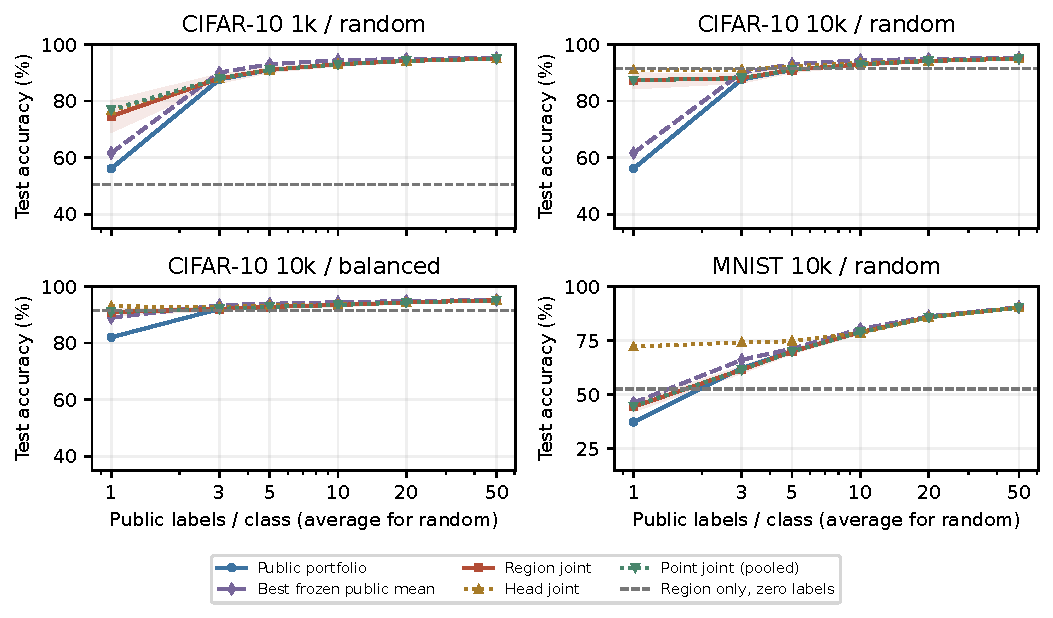
\includegraphics[width=.72\textwidth]{figures/fig-joint-frontier.pdf}
\Description{Matched public label budgets under random and balanced acquisition,
with public learning and identically decoded private release objects.}
\caption{Label access changes the comparison. Random panels use independent
confirmation cohorts/labels; balanced uses protocol cohorts. All private
arms release once at $\varepsilon=.1$ after 180 private steps. Public envelope
is descriptive over fourteen frozen learners; the portfolio is a LOO rule.
Private joint curves are ungated. All fitting/selection labels are inside m.
Shading is crossed pointwise bootstrap; text gives simultaneous intervals.}
\label{fig:label-frontier}
\end{figure*}

\begin{figure*}[t]
\centering
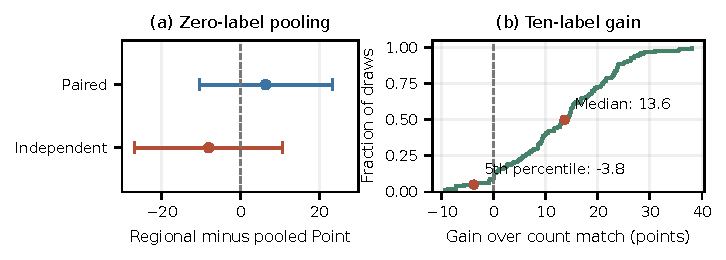
\includegraphics[width=.68\textwidth]{figures/fig-value-mechanisms-print.pdf}
\Description{Zero-label regional-minus-pooled differences reverse across two
cohort groups; ten-label gains have a positive median and a negative lower tail.}
\caption{CIFAR-1k, $\varepsilon=.1$. (a) Zero-label centered NN: regional/pooled
Point means are $52.2/45.8\%$ in paired cohorts and $50.3/58.4\%$ in independent
cohorts. Paired Student intervals use ten seeds per group. (b) Each label-mean
gain averages ten independent-confirmation cohorts against fixed raw-count
public matching. The 100 draws have mean \JointGain{}, median \GainMedian{}
and fifth percentile \GainFifth{} points. Crossed cases are not independent.}
\label{fig:value-mechanisms}
\end{figure*}

\subsection{What to buy: annotation access and the gain distribution}
\label{sec:eval:main}
\label{sec:eval:frontier}

With balanced labels (50 draws; the artifact tabulates all fourteen public
learners), three supplied
labels per class name the fixed CIFAR partition at $91.59\%$ in all 50 draws
(graph propagation: $92.61\%$), and ten feature-directed annotations recover
the same classifier without private reports. On MNIST's less class-aligned
regions one label per class gives $38.28\%$ majority naming versus
$58.36\%$ graph propagation.

Under passive random access, independent CIFAR-1k with ten labels gives
$61.62\%$ for the strongest mean public learner (raw-count matching) and
$74.62\%$ for joint naming (Figure~\ref{fig:label-frontier}). The
\JointGain{}-point mean gain has simultaneous interval \JointGainCI{}. The
median label-mean gain is \GainMedian{} points, so a few large draws do not
drive it; its fifth percentile is \GainFifth{}, and \GainNegativeDraws{}\% of
label means and \GainNegativeCases{}\% of label/cohort cases are negative
(Figure~\ref{fig:value-mechanisms}(b)). Label- and cohort-mean SDs are
\LabelAxisSD{}/\CohortAxisSD{} points.

Every ten-label CIFAR draw omits a class (30/50 labels: $31/7\%$), and the
public class-check rule rejects private augmentation at every tested budget,
so $74.62\%$ is an ungated utility (the artifact tabulates all fallbacks).
Random-only access is an experimental contract, not a known constraint of
CIFAR or Usenet. LOO selection contributes its own variation: the public
portfolio gives $56.13\%$ versus fixed count matching's $61.62\%$, and at
CIFAR-10k joint selection gives $87.35\%$ versus fixed zero-label private
naming's $91.59\%$ (Section~\ref{sec:eval:ceiling}).

\paragraph{A weaker encoder}
A frozen design replaces DINOv2 by an ImageNet ResNet-18 and reruns the
independent CIFAR-1k comparison with the same images, cohorts, label draws,
learners and release. The partition ceilings fall to
\EncCeilOne{}/\EncCeilMany{}\%. Ten feature-directed labels again reach the
one-to-one ceiling without private reports (\EncDirected{}\%); with ten
random labels, joint naming (\EncJoint{}\%) changes the strongest public
learner (\EncPublic{}\%) by \EncGain{} points (\EncGainCI{}). The registered
E1, a positive passive-access gain, fails; E2, directed labels beating random
labels plus private reports, holds. Under both encoders acquisition decides
whether private reports are needed; their passive-access value also needs
regions that carry the classes (Section~\ref{sec:eval:ceiling}).

\subsection{What to release: sensitivity versus accuracy}
\label{sec:eval:rounds}

Per-example votes are $\sqrt{|P|/K}$ times more sensitive than regional
reports (Section~\ref{sec:threat}); at $|P|=2000$ and $K=10$ the factor is
about 14, and they carry 20000 rather than 100 coordinates per client,
against 1280 for a head. Table~\ref{tab:joint-controls} holds
post-processing fixed: all three objects feed the same joint decoder and LOO
selection with the same labels (I/P: independent/paired cohorts; Public:
strongest of the fourteen public learners; Native Head uses no labels). Pooled point and regional joint naming differ
by at most \PointRegionMaxGap{} points on all \PointRegionSettings{} settings
(CIFAR-1k: $76.94$ versus $74.62\%$), while the head, whose native
predictions the partition does not bound, wins where the partition limits
regional naming (MNIST-10k: \HeadMnistTenK{} versus \RegionMnistTenK{}\%; at
CIFAR-10k native Head gives $94.0\%$). Published designs run through the same
protected sum in the inherited three-release protocol ($10^4$ clients,
$\varepsilon=.1$, \ExtSeeds{} seeds, publicly configured settings): on
CIFAR-10, DP-FedCT's per-example votes, our Point interface, reach
\ExtFedCTCifar{}\% and PATE-DI's screened teacher votes (RDP conversion)
\ExtPATECifar{}\%, against \ExtSDDCifar{}\% for regional reports and
\ExtHeadCifar{}\% for the clipped DP-Head (MNIST: \ExtFedCTMnist{},
\ExtPATEMnist{}, \ExtSDDMnist{} and \ExtHeadMnist{}\%).

Pooling explains why the sensitivity gap does not reach accuracy. Relative
to regional noise, averaging independent point noise in
region k has standard-deviation ratio approximately
\begin{equation}
\frac{v_{\mathrm{point,pool},k}}{v_{\mathrm{region}}}
\simeq\sqrt{\frac{|P|}{K |P_k|}}.
\label{eq:pooling-ratio}
\end{equation}
CIFAR's region sizes give ratios .88--1.07: pooled point votes carry about the
regional noise. At zero labels, CIFAR-1k regional-minus-pooled paired
differences are $+6.39$ points ($[-10.48,23.26]$) in protocol cohorts and
$-8.02$ ($[-26.81,10.77]$) in independent cohorts
(Figure~\ref{fig:value-mechanisms}(a)); neither supports a stable regional
advantage. The $\sqrt{|P|/K}$ ratio is a payload and interface property, not
an accuracy guarantee.

With fixed 60-step teachers, T=1 raises CIFAR-1k from $26.86\%$ to
$49.56\%$; no-feedback T=3 controls show no universal feedback penalty. The
pooling, round and no-feedback tables are in the artifact.

\subsection{What evidence to buy: mean gain versus class evidence}
\label{sec:eval:verification}

The verification demonstration (Table~\ref{tab:setup}, Verif.) uses ten new
CIFAR-1k cohorts, 100 fresh ten-label draws and an 80/20 source split
between training and held-out records. The comparator is raw-count matching;
candidates (eight joint weights, fixed private and public count rules) are
chosen from protected naming and the ten labels. Each of the 3000 cases
charges all three releases to one total budget; every utility is
unconditional, a rejection scoring its public fallback.

\paragraph{A cost ladder of publication targets}
Table~\ref{tab:verify-ladder} evaluates practical targets on these protected
outputs (acceptance / unconditional test accuracy; each row is a separately
declared rule with its own $\alpha=.025$ class family). Gain-only acceptance is \TightGlobalAccept{}\% at $\varepsilon=.1$
and \MiddleGlobalAccept{}\% at $\varepsilon=1$, where direct class-sum bounds
accept \MiddleClassAccept{}\% (initial coordinate-wise bands: zero). At $\varepsilon=3$, class-checked acceptance reaches
\LargerClassAccept{}\% ($86.63\%$ test accuracy against $62.30\%$ public), a
budgeted route to classwise evidence, not a validation of the $74.62\%$
classifier at unchanged privacy. A mean gain of at least $.20$ still accepts
\LadderGainTwoTenth{}\% of cases at $\varepsilon=1$. All-class recall of at
least $.25$ is accepted in \LadderRecallQuarterThree{}\% of cases at
$\varepsilon=3$, and $.50$ at no tested budget. Per-class non-degradation
against the comparator, $\mathrm{recall}_{f,c}-\mathrm{recall}_{b,c}\ge-\eta$,
depends on its tolerance: at $\varepsilon=3$ it accepts
\LadderNondegQuarter{}\% at $\eta=.25$ but \LadderNondegHalf{}\% at
$\eta=.5$; its band radius must fall below $\eta$ times a class mass of order
$1/C$. Costs are ordered only for stated thresholds. Gain-policy false accepts are 1/1000 at $\varepsilon=.1$, and no ladder rule
records one at $\varepsilon\ge1$.

\paragraph{What the cheap target publishes}
A correct mean-gain certificate says nothing about the worst class
(Figure~\ref{fig:verification}(a)). At $\varepsilon=1$ the mean-gain rule
publishes \MinRecGainOnePub{} of 1000 cases; \MinRecGainOneZero{}\% of them
recall some class below $1\%$ and \MinRecGainOneTenth{}\% below $10\%$
(\MinRecGainThreeTenth{}\% at $\varepsilon=3$). Every classifier the
all-recall rule publishes recalls each class above $50\%$; the ladder's price
difference buys exactly this tail.

\begin{table}[t]
\caption{Verification-Cost Ladder of Publication Targets}
\label{tab:verify-ladder}\small
\centering
\begin{tabular}{@{}lrrr@{}}\toprule
Publication target & $\varepsilon=.1$ & $\varepsilon=1$ & $\varepsilon=3$ \\
\midrule
gain $>0$ & 4.6 / 63.7 & 86.8 / 88.9 & 87.0 / 88.9 \\
gain $\ge.10$ & 2.2 / 63.0 & 82.0 / 88.2 & 85.0 / 88.7 \\
gain $\ge.20$ & 0.7 / 62.6 & 58.2 / 83.4 & 64.6 / 85.1 \\
all recalls $>0$ & 0.0 / 62.3 & 6.2 / 64.3 & 75.9 / 86.6 \\
all recalls $\ge.25$ & 0.0 / 62.3 & 0.0 / 62.3 & 75.7 / 86.6 \\
all recalls $\ge.50$ & 0.0 / 62.3 & 0.0 / 62.3 & 0.0 / 62.3 \\
non-degr. $\eta=.25$ & 0.0 / 62.3 & 0.0 / 62.3 & 2.0 / 63.2 \\
non-degr. $\eta=.50$ & 0.0 / 62.3 & 0.0 / 62.3 & 83.1 / 87.8 \\
\bottomrule\end{tabular}
\end{table}


\paragraph{Protocol price versus target price}
The ladder fixes one protocol: a $50/25/25$ split, both reports released and
two-sided bands. Table~\ref{tab:cost} varies each choice on draws 50--99.
\emph{Tight} applies one-sided lower bands to the same histograms (all-recall
acceptance at $\varepsilon=1$: \CostFixedRecallOne{}\% to
\CostTightRecallOne{}\%, nothing else changes); \emph{Re-rel.} re-releases
the stored clean statistics with fresh exact noise after reconstructing all
3000 histograms bit for bit; \emph{Opt.} uses the naming share $\phi$ that
maximized offline test accuracy on draws 0--49 (gain: $\phi$ to naming, the
rest to the gain report; classes: the gain report takes a quarter of the
rest). Both phases score the same test set and cohorts, so \emph{Opt.} is a
retrospective sensitivity analysis: the fixed split is far from best for class
targets ($\phi=\CostOptRecallOnePhi$: \CostRefRecallOne{}\% to
\CostOptRecallOne{}\% at $\varepsilon=1$), so Table~\ref{tab:verify-ladder}
prices one protocol, not the targets.

\begin{table}[t]
\caption{Verification Cost under Four Protocols}
\label{tab:cost}\small\setlength{\tabcolsep}{1.6pt}
\centering
\begin{tabular}{@{}llrrrrrr@{}}\toprule
Target & $\varepsilon$ & Fixed & Tight & Re-rel. & Opt. & $\phi$ & Disjoint \\
\midrule
gain $>0$ & .1 & 5.4/64.5 & 5.4/64.5 & 6.6/64.6 & 12.4/66.4 & .4 & 5.0/64.2 \\
 & 1 & 88.0/90.3 & 88.0/90.3 & 88.0/90.3 & 88.0/90.2 & .1 & 88.0/90.2 \\
 & 3 & 88.0/90.3 & 88.0/90.3 & 88.0/90.5 & 88.2/90.5 & .5 & 88.4/90.6 \\
all recalls $>0$ & .1 & 0.0/62.8 & 0.0/62.8 & 0.0/62.8 & 0.0/62.8 & -- & 0.0/62.8 \\
 & 1 & 6.4/64.9 & 19.8/69.0 & 7.8/65.2 & 81.8/88.5 & .1 & 7.4/65.1 \\
 & 3 & 82.8/89.0 & 82.8/89.0 & 83.6/89.5 & 83.6/89.3 & .3 & 84.2/89.6 \\
all recalls $\ge.50$ & .1 & 0.0/62.8 & 0.0/62.8 & 0.0/62.8 & 0.0/62.8 & -- & 0.0/62.8 \\
 & 1 & 0.0/62.8 & 0.0/62.8 & 0.0/62.8 & 0.0/62.8 & -- & 0.0/62.8 \\
 & 3 & 0.0/62.8 & 0.0/62.8 & 0.0/62.8 & 70.2/85.0 & .1 & 0.0/62.8 \\
\bottomrule\end{tabular}
\end{table}


\paragraph{Choosing the split before deployment}
Can a platform find such a split without the test set? A third frozen
design splits the 45000 private CIFAR images per class into two pools; ten
\emph{development} cohorts come from one and ten \emph{confirmation}
cohorts from the other, each with 1000 clients holding \BCRecTrain{}
training and \BCRecHeld{} held-out records used once. On development cohorts
and label draws 0--49, each target and budget gets the grid $\phi$ that
maximizes the accuracy of the published classifier on the labelled public
validation split; the selection reads only protected decisions and
validation labels and was frozen before any confirmation case ran. Confirmation cohorts, label
draws 50--99 and the test split then compare the frozen share with the fixed
split at the same total budget (Table~\ref{tab:budgetconf},
\BCCases{} cases; $\Delta$ with crossed-bootstrap 95\% interval, FA false
accepts, Best the unused confirmation-best share). The pre-registered primary test holds: at
$\varepsilon=1$, all-recall acceptance rises from \BCFixedRecallOne{}\% to
\BCFrozenRecallOne{}\% ($\BCDiffRecallOneAcc$ points, $\BCDiffRecallOneAccCI$)
and test accuracy from \BCFixedRecallOneUtil{} to \BCFrozenRecallOneUtil{}\%
($\BCDiffRecallOneUtil$, $\BCDiffRecallOneUtilCI$). Recall $\ge.5$ becomes
certifiable at $\varepsilon=3$ (\BCFrozenHalfThree{}\% acceptance,
\BCFrozenHalfThreeUtil{}\% accuracy), mean-gain cells move by at most
\BCGainMaxDiff{} points, and no frozen cell records a false accept.
Development and confirmation curves agree
(Figure~\ref{fig:verification}(b,c)); the frozen share loses at most
\BCMaxRegret{} points to the confirmation-best one. The registered prediction
that class shares fall below $.5$ at $\varepsilon\le1$ failed only where no
share certifies anything and ties default to $.5$. One development cohort
with ten draws already selects well (\BCPilotRecallOne{}\% confirmation
accuracy at $\varepsilon=1$, \BCPilotHalfThree{}\% for recall $\ge.5$ at
$\varepsilon=3$, mean of \BCPilotSubsamples{} such pilots). The pilot is a
separate population with its own ledger: \PilotDevLabels{} development labels
(ten draws of ten), the \PilotValLabels{} public validation labels that score
each published classifier, and \PilotReleases{} protected releases over
\PilotConfigs{} grid configurations. Answered by one population they compose
to \PilotRhoMult{} times a deployment's zCDP budget (total
$\varepsilon\approx\PilotEpsOne{}$ for deployments at $\varepsilon=1$). The
deployment's public learners do not see the pilot's labels; a platform allowed
to train on its validation labels should compare against learners that do.

\paragraph{Natural writers: an external test of the planner}
FEMNIST runs the same protocol (Table~\ref{tab:budgetconf}, lower block):
1000 writers per cohort from two disjoint pools, a seeded 80/20 split of each
writer's records ($H_i$ varies, median 32), 62 random labels, \FCCases{} cases.
Reports, certificates, clean statistics, planner inputs and false-accept
judgments all use the client-weighted statistics of Section~\ref{sec:problem}.
Planner predictions frozen before confirmation lie within \FCPlanGap{} points
of every cell, with no false accept; the cells sit near 0 or 100\%, so this
checks calibration at the extremes. The study prices verification, not
private value: the mean-gain rule accepts \FCGainOne{}\% at $\varepsilon=1$
against the \FCPub{}\% count-matching comparator, yet its \FCUtilFixed{}\%
stays below the strongest public learner on the same labels
(\FCPublicBest{}\%) and \FCTail{}\% of what it publishes recalls some class
below 10\%. Candidates miss whole classes, so no class target is certifiable
and the split cannot help, as the planner predicted.

\begin{table*}[t]
\caption{Budget Split Selected on Development Cohorts and Confirmed on New Cohorts}
\label{tab:budgetconf}\small\setlength{\tabcolsep}{4pt}
\centering
\begin{tabular}{@{}lllrrrrrrr@{}}\toprule
Task & Target & $\varepsilon$ & $\phi$ & Fixed & Frozen & Planner & $\Delta$ accuracy & FA & Best \\
\midrule
CIFAR & gain $>0$ & .1 & .3 & 3.8/63.8 & 4.0/63.8 & -- & +0.0 [$-$1.0, +1.0] & 0 & .5 \\
 &  & 1 & .5 & 88.0/90.2 & 87.6/90.0 & -- & $-$0.1 [$-$0.7, +0.2] & 0 & .6 \\
 &  & 3 & .2 & 88.0/90.6 & 88.0/90.6 & -- & +0.0 [$-$0.2, +0.2] & 0 & .4 \\
 & all recalls $>0$ & .1 & .5 & 0.0/62.8 & 0.0/62.8 & -- & +0.0 [+0.0, +0.0] & 0 & -- \\
 &  & 1 & .2 & 5.4/64.5 & 78.2/87.2 & -- & +22.8 [+18.9, +26.7] & 0 & .3 \\
 &  & 3 & .2 & 83.8/89.6 & 83.6/89.5 & -- & $-$0.1 [$-$0.8, +0.3] & 0 & .6 \\
 & all recalls $\ge.50$ & .1 & .5 & 0.0/62.8 & 0.0/62.8 & -- & +0.0 [+0.0, +0.0] & 0 & -- \\
 &  & 1 & .5 & 0.0/62.8 & 0.0/62.8 & -- & +0.0 [+0.0, +0.0] & 0 & -- \\
 &  & 3 & .1 & 0.0/62.8 & 76.2/87.2 & -- & +24.4 [+19.9, +28.6] & 0 & .1 \\
\midrule
FEMNIST & gain $>0$ & 1 & .9 & 99.0/35.1 & 98.2/35.2 & 98.7/98.1 & +0.0 [$-$0.7, +0.6] & 0 & .7 \\
 &  & 3 & .2 & 100.0/35.5 & 100.0/35.5 & 99.3/99.7 & +0.0 [$-$0.6, +0.5] & 0 & .3 \\
 &  & 10 & .1 & 100.0/35.1 & 100.0/35.1 & 100.0/100.0 & +0.0 [$-$0.2, +0.3] & 0 & .3 \\
 & all recalls $>0$ & 1--10 & .5 & 0.0/11.6 & 0.0/11.6 & 0.0/0.0 & +0.0 [+0.0, +0.0] & 0 & -- \\
 & all recalls $\ge.50$ & 1--10 & .5 & 0.0/11.6 & 0.0/11.6 & 0.0/0.0 & +0.0 [+0.0, +0.0] & 0 & -- \\
\bottomrule\end{tabular}
\end{table*}


\begin{figure*}[t]
\centering
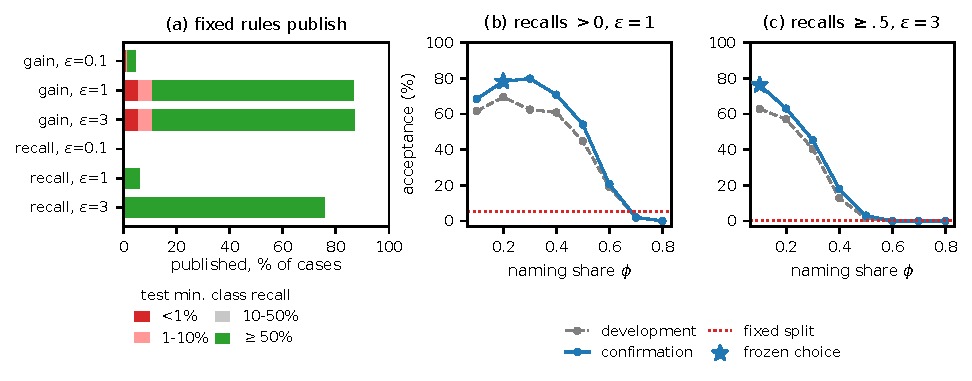
\includegraphics[width=.9\textwidth]{figures/fig-verification-print.pdf}
\Description{Minimum test class recall of classifiers published by the fixed
rules, and development versus confirmation acceptance over the naming share.}
\caption{(a) The 1000 cases per budget of Table~\ref{tab:verify-ladder}, by
the test minimum class recall of the classifier each fixed rule publishes
(offline diagnostic). (b, c) Acceptance over the naming share $\phi$ on the
development cohorts (dashed, used for selection) and the confirmation
cohorts (solid); the star is the frozen choice and the dotted line the fixed
$50/25/25$ split on the confirmation cohorts.}
\label{fig:verification}
\end{figure*}

\paragraph{Source-disjoint clients}
Constructed CIFAR clients in the ladder reuse source images. A design frozen
before implementation rebuilds the ladder on ten new cohorts in which each of
\DisjSources{} private images belongs to one client, \DisjRecords{} for
training and \DisjHeld{} held out, with the same candidates, labels, split and
bands (Table~\ref{tab:cost}, Disjoint). The mean top-class share is \HetDisjoint{}
(last 100 clients \HetLast{}; \HetReused{} with reuse). The gain
policy beats the fallback by \DisjGainImpr{} points at $\varepsilon=1$
(\DisjGainCI{}; \ReusedGainImpr{} with reuse) and every rung stays within
\DisjMaxDiff{} points; the predicted shrinkage did not occur. Its two false
accepts at $\varepsilon=3$ have true gain zero, within $\alpha$.
Disjointness also cuts records per client, so this does not show that
reuse is irrelevant.

\paragraph{A planning map beyond the tested setting}
Per case, the calculator takes the clean gain $g$, class masses $m_c$,
recalls $r_c$ and differences $d_c$. Treating each report as Gaussian with its calibrated std ($2v_g$ for the
gain, $v_h$ per coordinate) and keeping rounding terms, it returns $\Phi((g-a_g-\gamma)/2v_g)\prod_c\Phi(\mu_c/\sigma_c)$,
with $a_g$ the gain band radius. A class rule accepts when a linear statistic
of class $c$ clears zero: for recall $\ge r_0$, $N^L_c-r_0D^U_c\ge0$, so
$\mu_c=r_cm_c-a_N-r_0(m_c+a_D)$ and $\sigma_c=v_h\sqrt{2(1-r_0)^2+2r_0^2}$
(Eq.~\eqref{eq:hist-radius}); for non-degradation, $\mu_c=(d_c+\eta)m_c$
minus its radius and $\sigma_c=v_h\sqrt{2+4\eta^2}$. The linear statistics
ignore the clipping of the bands. Capping $D^U_c$ at 1 can only raise
acceptance and binds only when the released class mass exceeds $1-a_D$
(probability $\Phi((m_c+a_D-1)/2v_h)$); clipping at zero changes a decision
only when that mass falls below $-a_D$. Outside these events the linear form
is exact. Classes and reports multiply because their noise is independent. The
result is an approximate planning quantity, not a coverage guarantee. It reproduces
all \CalcCells{} rates of Table~\ref{tab:verify-ladder} within \CalcGap{}
points; frozen before the new-cohort study of Section~\ref{sec:eval:ceiling},
it also matches its \PlanOOSCells{} gain and class rates (other $n$, $C$ and
natural Usenet clients, class masses \UsenetMassMin{}--\UsenetMassMax{})
within \PlanOOSGap{} points. This validates the noise calibration, not
effect sizes. At the median CIFAR-1k effect sizes, the artifact's planning
map gives the smallest total $\varepsilon$ accepting each target with
probability one half; as $v\propto1/(n\sqrt\rho)$, the
required $\rho$ scales as $n^{-2}$ and $\varepsilon$ roughly as $1/n$. It is
conditional on effect sizes: at $n=10$k it prices all recalls $>0$ at
\PlanRecallZeroNTenK{}, yet the new MNIST candidates, with a nearly empty
worst class, pass in \MnistClassOne{}\% of cases at $\varepsilon=1$.

\subsection{Explaining the losses: partition ceilings}
\label{sec:eval:ceiling}

\begin{table*}[t]
\caption{Where Regional Value Is Lost}
\label{tab:decomposition}\small\setlength{\tabcolsep}{3.2pt}
\centering
\begin{tabular}{@{}lrrrrrrrrrrrrr@{}}\toprule
Task/$\varepsilon$ & Ceil. & Pub. & Room & Clean & Named & Joint & $\Delta_T$ & $\Delta_N$ & $\Delta_S$ & N$\uparrow$ & $v$ & Gated & Head \\
\midrule
CIFAR 1k/0.1 & 91.6/91.6 & 61.6 & +30.0 & 91.6 & 50.3 & 74.6 & +0.0 & +41.2 & -24.3 & 0/10 & 0.215 & 74.6 & 76.6 \\
CIFAR 10k/0.1 & 91.6/91.6 & 61.6 & +30.0 & 91.6 & 91.6 & 87.4 & +0.0 & +0.0 & +4.2 & 0/10 & 0.022 & 91.6 & 91.1 \\
MNIST 10k/0.1 & 52.6/54.1 & 46.2 & +7.9 & 53.9 & 52.6 & 44.4 & +0.2 & +1.3 & +8.2 & 2/10 & 0.022 & 52.6 & 72.2 \\
Usenet 3k/1 & 42.4/42.5 & 32.1 & +10.3 & 32.3 & 20.7 & 28.2 & +10.2 & +11.6 & -7.5 & 0/10 & 0.006 & 21.0 & 31.8 \\
FEMNIST 1k/0.1 & 24.6/42.9 & 37.3 & +5.5 & 35.3 & 7.1 & 36.0 & +7.5 & +28.3 & -28.9 & 0/10 & 0.535 & 36.0 & 36.0 \\
FEMNIST 1k/1 & 24.6/42.9 & 37.3 & +5.5 & 35.3 & 35.5 & 35.9 & +7.5 & -0.2 & -0.4 & 5/10 & 0.055 & 35.9 & 38.1 \\
FEMNIST 2k/0.1 & 24.6/42.9 & 37.3 & +5.5 & 35.3 & 19.8 & 36.0 & +7.5 & +15.5 & -16.2 & 0/10 & 0.268 & 36.0 & 35.9 \\
FEMNIST 2k/1 & 24.6/42.9 & 37.3 & +5.5 & 35.3 & 35.6 & 35.8 & +7.5 & -0.2 & -0.2 & 6/10 & 0.027 & 35.6 & 38.5 \\
\bottomrule\end{tabular}
\end{table*}

% Data figure, generated by export_eab13.py (figures/fig-ceiling-print.pdf): audit panel of the former fig-ceiling;
% its decomposition panel duplicated Table VIII and remains in figures/fig-ceiling.pdf (artifact).
\begin{figure}[t]
\centering
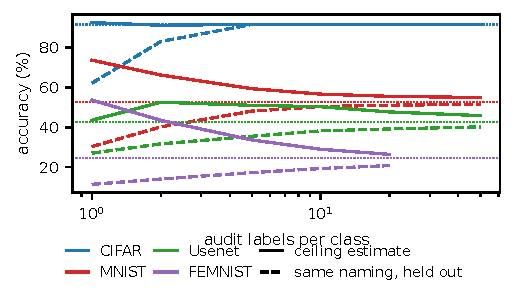
\includegraphics[width=\columnwidth]{figures/fig-ceiling-print.pdf}
\Description{Audit-sample ceiling estimates versus held-out naming accuracy.}
\caption{Auditing the ceiling. A random labelled audit of the development
split: its in-sample one-to-one ceiling estimate (solid) and the test accuracy
of the naming it induces (dashed); dotted lines are the true ceilings; 200
repetitions. Offline diagnostic.}
\label{fig:ceiling}
\end{figure}


A regional readout assigns one class per public region, so its accuracy is
bounded by the \emph{partition ceiling}, the best such assignment within the
decoder's family: $\mathrm{Ceil}_{1:1}$ for
assignment decoders, $\mathrm{Ceil}_{M:1}\ge\mathrm{Ceil}_{1:1}$ for centered
decoding. With $P^\star$ the strongest public learner, the regional part of
the marginal value in Eq.~\eqref{eq:marginal-value} for decoder family $D$
satisfies
\begin{equation}
V^{\mathrm{reg}}_D\le\mathrm{Ceil}_D-P^\star .
\label{eq:ceiling}
\end{equation}
The stored clean vote matrices, never released, make the gap below the
ceiling measurable. Decoding them with the centered decoder of the protected
release gives \emph{noise-free naming} $N_0$; with protected naming
$N_\varepsilon$ and joint selection $J$, on one partition, decoder, data and
seed set,
\begin{equation}
\mathrm{Ceil}_{M:1}-J=\underbrace{\mathrm{Ceil}_{M:1}-N_0}_{\Delta_T}
+\underbrace{N_0-N_\varepsilon}_{\Delta_N}
+\underbrace{N_\varepsilon-J}_{\Delta_S}
\label{eq:decomposition}
\end{equation}
The identity telescopes, so its terms are signed controlled differences, not
causal attributions: noise improves naming on \NoiseImprMnist{} MNIST seeds
and \NoiseImprFemnist{} FEMNIST-2k/1 seeds, and $\Delta_S$ is negative
wherever fusion with the labels corrects noisy names ($\SelCifarOne$ points
on CIFAR-1k). We read $\Delta_T$ as teacher content, $\Delta_N$ as release
noise and $\Delta_S$ as selection only where a term is large and stable
across seeds (Table~\ref{tab:decomposition};
Room is $\mathrm{Ceil}_{M:1}-P^\star$, N$\uparrow$ counts seeds where noise
improves naming, $v$ is the naming-noise std).

\emph{Teacher content} bounds the natural-client tasks. Usenet has
\RoomUsenetMany{} points of room, but noise-free naming reaches only the
public level, \CleanUsenet{}\% ($\Delta_T=\TeachUsenet$): votes barely
differ between regions, so even small noise ($v=\NoiseUsenet$) flips
most regions and costs another \NoiseLossUsenet{} points. On FEMNIST no
assignment decoder can add value (one-to-one ceiling \CeilFemnistOne{}\%,
below public); the many-to-one ceiling leaves \RoomFemnistMany{} points, and
noise-free naming reaches \CleanFemnist{}\% ($\Delta_T=\TeacherFemnist$),
which protected naming matches at $\varepsilon=1$. \emph{Release noise} adds
\NoiseLossFemnistTenth{}--\NoiseLossFemnistOneTenth{} points on FEMNIST at
$\varepsilon=.1$ and \NoiseLossCifarOne{} points on CIFAR-1k
($v=\NoiseCifarOne$), where clean naming is at the ceiling and joint fusion
with ten labels recovers $74.62\%$. \emph{Selection} is the dominant term where
protected naming already realizes the room. On CIFAR-10k ($v=\NoiseCifarTen$)
fixed protected naming reaches the ceiling, \NamedCifarTen{}\%, and LOO
loses \SelLossCifarTen{} points. On MNIST the many-to-one ceiling is
\CeilMnistMany{}\%; $\Delta_T=\TeachMnist$, $\Delta_N=\NoiseMnist$ and
$\Delta_S=\SelMnist$, turning a \RoomMnistMany{}-point room into a negative
joint gain, while the head, which the partition does not bound, reaches
\HeadMnist{}\% (Section~\ref{sec:eval:rounds}).

\paragraph{An exploratory selection rule}
Random $m=C$ draws almost always miss a class, and LOO then compares
candidates on classes it cannot see. After earlier rounds, we registered a
rule family: LOO; keep protected naming whenever labels miss a class; or do
so only if also the public noise scale $v(n,\varepsilon,K)\le v_0\in
\{.01,.03,.1\}$. One rule is selected on draws 0--49 and evaluated on draws
50--99 of the same cohorts, an exploratory estimate. The coverage-only rule fails where noise
is large ($\CoverCifarOne$ points on CIFAR-1k). The
selected rule, $v_0=\GateVzero$, raises the held-out gain over the strongest
public learner from $\LooMnistHeld$ to $\GatedMnistHeld$ points on MNIST and
from $\LooCifarTenHeld$ to $\GatedCifarTenHeld$ on CIFAR-10k, but lowers
Usenet from $\LooUsenetHeld$ to $\GatedUsenetHeld$: its noise is the smallest,
and the rule cannot see its poor teacher. No tested rule dominates; choosing privately would be private selection
\cite{liu2019private}.

\paragraph{Private verification screens the gated candidate}
A frozen design runs on new cohorts (\VTSeeds{} per task, \VTCases{}
cases): the gated rule names a candidate, the LOO portfolio is the
comparator, and disjoint holdout clients release gain and class histogram
under one $50/25/25$ budget. At $\varepsilon=1$ the gate is open and its
sign replicates ($\VTMnistGatedLoo$ points over LOO
on MNIST, $\VTUsenetGatedLoo$ on Usenet; Table~\ref{tab:verify-teacher}, whose
acceptance and false accepts (FA) count cases with a private candidate, Priv.).
Verification accepts \VTMnistAccept{}\% of private candidates on MNIST and
\VTCifarAccept{}\% on CIFAR-10k with no false accept in any case, so the
verified rule keeps the MNIST gain ($\VTMnistVerLoo$ $\VTMnistVerLooCI$)
and returns Usenet's mean balanced accuracy to the LOO level
($\VTUsenetVerLoo$ $\VTUsenetVerLooCI$), without a per-case guarantee.
The pre-registered task-level criterion, at most $10\%$ acceptance on
Usenet, was not met: \VTUsenetAccept{}\% of its \VTUsenetPriv{} private
candidates were accepted. Verification separates cases, not tasks. Post hoc,
the \VTUsenetAccepted{} accepted Usenet cases gain $\VTUsenetAccAcc$ test
accuracy points and the rejected ones $\VTUsenetRejAcc$ (draws where the
six-label portfolio is weak), but the target is client-mean accuracy and
accepted cases gain only $\VTUsenetAccBal$ balanced points
(\VTUsenetAccBalShare{}\% positive). A balanced-accuracy rule
on the same released histogram, added after the outcome, accepts
\BalUsenetAccept{}\% on Usenet and \BalMnistAccept{}\% on MNIST
(Table~\ref{tab:verify-teacher}): the verified target, not the verifier,
decides whether Usenet publishes. No MNIST candidate meets the all-class
recall target at this budget.

\begin{table}[t]
\caption{Gated Rule plus Private Verification on New Cohorts}
\label{tab:verify-teacher}\small\setlength{\tabcolsep}{2.2pt}
\centering
\begin{tabular}{@{}lrrrrrrrrr@{}}\toprule
 & & \multicolumn{2}{c}{Accept} & & & & & \multicolumn{2}{c}{Verified} \\
Task & Priv. & acc & bal & FA & Pub. & LOO & Gated & acc & bal \\
\midrule
MNIST 10k & 500 & 99.6 & 77.4 & 0 & 37.3 & 43.0 & 53.6 & 53.6 & 52.3 \\
CIFAR 10k & 500 & 98.0 & 98.0 & 0 & 55.9 & 88.0 & 91.6 & 91.6 & 91.6 \\
Usenet 3k & 495 & 20.6 & 0.0 & 0 & 28.2 & 28.2 & 23.8 & 28.7 & 28.2 \\
\bottomrule\end{tabular}
\end{table}


\paragraph{Auditing the ceiling is public naming}
Estimating the one-to-one ceiling from a labelled audit finds the best
assignment on its confusion matrix, so the estimate is the in-sample accuracy
of the naming the audit induces. Figure~\ref{fig:ceiling} compares the two
on audits from the development split; test labels only score.
With one label per class, the CIFAR estimate is \AuditCifarOneEst{}\% while
the induced naming achieves \AuditCifarOneHeld{}\% on test; at five per
class they meet at \AuditCifarFiveEst{}/\AuditCifarFiveHeld{}\%, the
ceiling. The others converge more slowly (MNIST and Usenet at 50 per class:
\AuditMnistFiftyEst{}/\AuditMnistFiftyHeld{}\% and
\AuditUsenetFiftyEst{}/\AuditUsenetFiftyHeld{}\%, one-to-one ceilings
\CeilMnist{}/\CeilUsenet{}\%). The estimate became accurate only once the
induced naming was itself near the ceiling, so the ceiling is an
\emph{ex post} diagnostic.

\subsection{Natural writers and text clients}
\label{sec:eval:natural}

FEMNIST proxy purity rises from .361 at K=31 to .654 at K=500, but at 2k
writers finer regions help only at $\varepsilon=1$ (K=124: $38.63\%$ versus
$35.57\%$ at K=62) and hurt at $\varepsilon=.1$ (K=31/62/124:
$22.68/19.80/12.63\%$); 5000 public labels reach $50.65/59.33\%$ at
180/600 steps. Usenet's public portfolio matches
or exceeds joint naming at every random-label budget (both $63.90\%$
balanced at 300 labels).
